\chapter{Pruebas simuladas con TORCS}
\label{ape:pruebasT}

\section{Atributos de los vehículos de TORCS}
\label{ape:atributos}

Los automóviles implementados por TORCS, son altamente personalizables, poseen una gran variedad de atributos que pueden modificarse, de manera que podemos generar una amplia gama de vehículos diferentes. En las figuras \ref{fig:c11}, \ref{fig:c8}, \ref{fig:c1} y \ref{fig:c6}, podemos observar algunos de los atributos que pueden configurarse.


\begin{figure}[h]
\vspace*{2 mm}
\begin{minipage}[b]{0.5\linewidth}
\centering
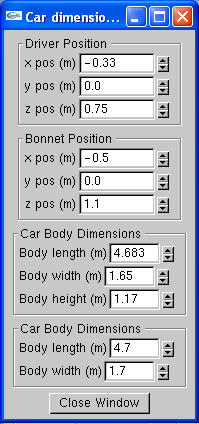
\includegraphics[scale= 0.5,type=png,ext=.png,read=.png]{figures/c11}
\caption{Dimensiones del carro.}
\label{fig:c11}
\end{minipage}
\begin{minipage}[b]{0.5\linewidth}
\centering
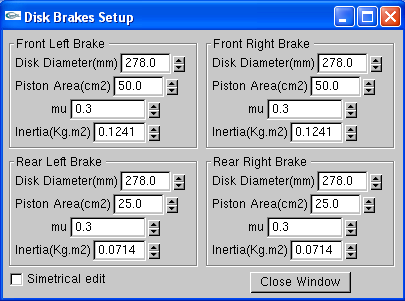
\includegraphics[scale= 0.5,type=png,ext=.png,read=.png]{figures/c8}
\caption{Discos de frenos.}
\label{fig:c8}
\end{minipage}
\end{figure} 

\begin{figure}[h]
\begin{minipage}[t]{0.5\linewidth}
\centering
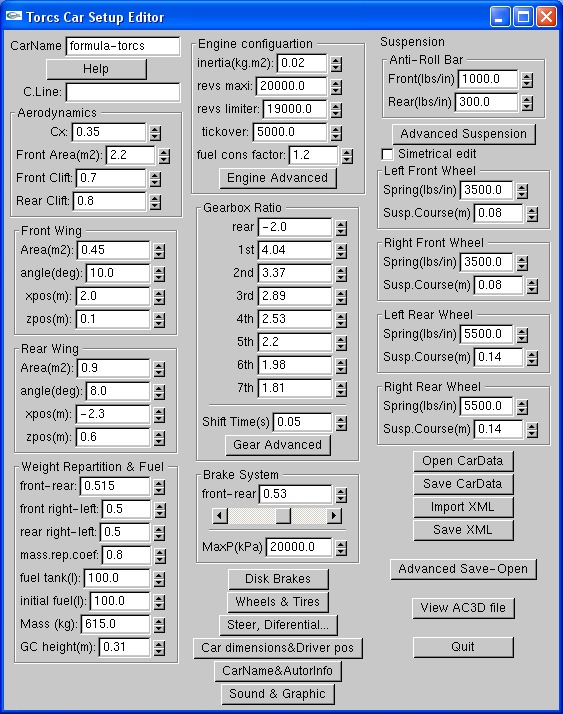
\includegraphics[scale= 0.45,type=png,ext=.png,read=.png]{figures/c1}
\caption{Configuración general.}
\label{fig:c1}
\end{minipage}
\hspace{0.5cm}
\begin{minipage}[t]{0.5\linewidth}
\centering
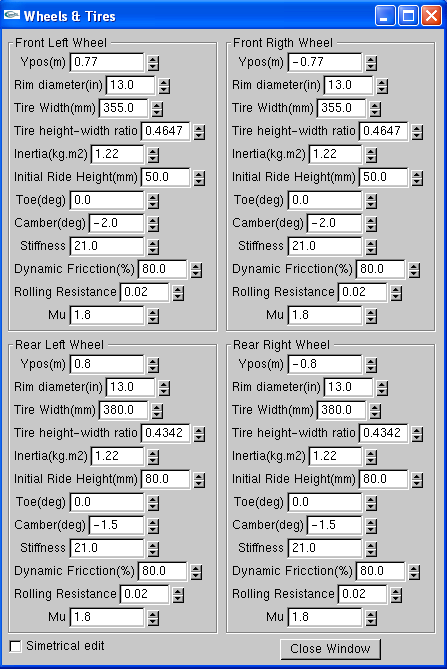
\includegraphics[scale= 0.45,type=png,ext=.png,read=.png]{figures/c6}
\caption{Ruedas y cauchos.}
\label{fig:c6}
\end{minipage}
\end{figure} 